%%%%%%%%%%%%%%%%%%%%%%%%%%%%%%%%%%%%%%%%%
% a0poster Portrait Poster for LiRI/UZH
% LaTeX Template
% Version 1.0 (22/06/13)
% Version 2.0 (08/04/22)
%
% The a0poster class was created by:
% Gerlinde Kettl and Matthias Weiser (tex@kettl.de)
% adapted by Danny McDonald for LiRI/UZH (mcddjx@gmail.com)
%
% License:
% CC BY-NC-SA 3.0 (http://creativecommons.org/licenses/by-nc-sa/3.0/)
%
%%%%%%%%%%%%%%%%%%%%%%%%%%%%%%%%%%%%%%%%%

\documentclass[a0,portrait]{a0poster}

% control margins here
\usepackage{geometry}
 \geometry{
 a0paper,
 left=5cm,
 top=4.5cm,
 right=5cm,
 bottom=4.5cm
 }
\addtolength{\textwidth}{4.5cm} % width of text can be adjusted if margins above are adjusted

\usepackage{multicol} % This is so we can have multiple columns of text side-by-side
\columnsep=3em % This is the amount of white space between the columns in the poster
\columnseprule=0pt % This is the thickness of the black line between the columns in the poster

% UZH colours
\usepackage[svgnames]{xcolor}
\definecolor{red100}{RGB}{204, 3, 1}
\definecolor{uzhblau80}{RGB}{51,83,183}
\definecolor{uzhockerrot100}{RGB}{220, 96, 39}
\definecolor{uzhockerrot80}{RGB}{227, 128, 82}
\definecolor{uzhflaschengruen100}{RGB}{42, 127, 98}
\definecolor{uzhflaschengruen80}{RGB}{86, 157, 133}
\definecolor{conclusion}{RGB}{204,212,237} % the conclusion box colour
\usepackage{multirow}

\usepackage{ifthen} % needed to stop horizontal line above 'Conclusions' section
\usepackage{graphicx} % Required for including images
\graphicspath{{figures/}} % Location of the graphics files
\usepackage{mwe,tikz}\usepackage[percent]{overpic} % overlay your photo over the background
\usepackage{booktabs} % Top and bottom rules for table
\usepackage[font=small,labelfont=bf]{caption} % Required for specifying captions to tables and figures
\usepackage{amsfonts, amsmath, amsthm, amssymb} % For math fonts, symbols and environments
\usepackage{wrapfig} % Allows wrapping text around tables and figures

\usepackage{fontspec} % custom fonts
\defaultfontfeatures[Palatino]
{
    Extension = .ttf,
    UprightFont = font/LT_41167,
    BoldFont = font/LT_41169,
    ItalicFont  = font/LT_41168,
    BoldItalicFont = font/LT_41170,
}
\defaultfontfeatures[TheSans]
{
    Extension = .otf,
    UprightFont = font/TheSans-LP5Plain,
    BoldFont = font/TheSans-LP7Bld,
    ItalicFont  = font/TheSans-LP5PlainIT,
    BoldItalicFont = font/TheSans-LP7BldIT,
}
\setmainfont{TheSans} % choose your font here
\usepackage[onehalfspacing]{setspace} % remove for single spacing
\usepackage{tcolorbox} % for the conclusions box
\usepackage{blindtext} % you can remove this once you add your content
\usepackage[export]{adjustbox} % allow floating a graphic right
\usepackage{titlesec} % customising section titles
\usepackage{needspace} % prevent break between line and section title
\usepackage{nameref} % package and command to get the name of the current section (for ifthen)

\begin{document}

% define how our section titles will look (with ruled line)
\titleformat{\section}
  {\needspace{1\baselineskip}\sectionrule\huge\bfseries}
  {\color{red100}\thesection.}
  {1em}
  {\color{red100}}

% draw horizontal line before section unless it is conclusions (if you change name of Conclusions, you should
% also change it here too so it is recognised and the line suppressed
\makeatletter
\newcommand{\sectionrule}{%
 \ifthenelse{\equal{\@currentlabelname}{Conclusions}}
 % use the below line instead of the above if conclusions is a section*
 % \ifthenelse{\equal{\@currentlabelname}{}}
  {}
  {\vspace*{-\baselineskip}
  %  \vrule height 1pt depth 1pt width \linewidth\vskip0.4pt
   \bigskip}%
}
\makeatother


%----------------------------------------------------------------------------------------
%	POSTER HEADER 
%----------------------------------------------------------------------------------------
%\title{Creating a \LaTeX{} poster template matching UZH specifications for LiRI presentations}
\title{PyPSA Energy Research Software}

% the top logo (in english!) and unit title
% \noindent

\noindent
\begin{minipage}[b][2cm][t]{0.74\linewidth} 
  % First Row
  \vspace{1em}
  \begin{minipage}{0.15\textwidth}
    
\includegraphics[height=3.5cm]{tub-logo.pdf}
  \end{minipage}
  \begin{minipage}{0.2\textwidth}
    
\includegraphics[height=4.5cm]{ensys-logo-en.pdf}
  \end{minipage}
  \vspace{6em}

  % Second Row
  \begin{minipage}{1\textwidth}
    \makeatletter
    \raggedright{\fontsize{80pt}{100pt}\selectfont\color{red100}\textbf{{\@title}}\par}
    \makeatother
    \color{Black}
    \vspace{0.2cm}
    \hspace{0.005em}
    www.pypsa.org
  \end{minipage}
\end{minipage}%
%
\begin{minipage}[b][2cm][t]{0.25\linewidth} % Second minipage
  
\includegraphics[width=0.7\textwidth]{qr-code.png} % Ensure correct width
  % \vspace{1em} % Add space below QR code, if needed
\end{minipage}

\vspace{17em}



%----------------------------------------------------------------------------------------
%	POSTER BODY
%----------------------------------------------------------------------------------------

\begin{multicols}{3}
\raggedcolumns

%----------------------------------------------------------------------------------------
%	PYPSA
%----------------------------------------------------------------------------------------
\noindent \textcolor{red100}{\huge \textbf{PyPSA}}
\\
\textit{Python for Power System Analysis}
\\

\noindent
PyPSA is an open-source toolbox for \textbf{simulating and optimising modern power and energy 
systems} that include features such as conventional generators with unit commitment, 
variable wind and solar generation, storage units, coupling to other energy sectors, 
and mixed alternating and direct current networks. \\

\noindent \textcolor{black}{\large \textbf{Functionality}}

\noindent PyPSA can calculate:

\begin{itemize}
    \item static power flow (using both the full non-linear network equations and the linearised network equations)
    \item linear optimal power flow (least-cost optimisation of power plant and storage dispatch within network constraints, using the linear network equations, over several snapshots)
    \item security-constrained linear optimal power flow
    \item total electricity/energy system least-cost investment optimisation
\end{itemize}


\noindent \textcolor{black}{\large \textbf{Components}}

\begin{itemize}
    \item meshed multiply-connected AC and DC networks, with controllable converters between AC and DC networks
    \item standard types for lines and transformers following the implementation in pandapower
    \item conventional dispatchable generators and links with unit commitment
    \item generators with time-varying power availability, such as wind and solar generators
    \item storage units with efficiency losses
    \item simple hydroelectricity with inflow and spillage
    \item coupling with other energy carriers (e.g. resistive Power-to-Heat (P2H), Power-to-Gas (P2G), battery electric vehicles (BEVs), Fischer-Tropsch, direct air capture (DAC))
    \item basic components out of which more complicated assets can be built, such as Combined Heat and Power (CHP) units and heat pumps
\end{itemize}

\vspace{2em}
\begin{tcolorbox}[width=0.95\linewidth,colback={conclusion},frame empty,boxsep=1cm]
\section*{Contribution}
  All tools are actively developed and maintained by the Department of Digital 
  Transformation in Energy Systems at the Technical University of Berlin and the 
  \textbf{PyPSA community}. Any contributions are welcome and can be made via GitHub. 
  Find contribution guidelines in the documentation for all tools. \\
  \\
  PyPSA is used by several research institutes, companies and non-governmental 
  organisations around the world. While much of this is proprietary work, several 
  notable model implementations are available as open-source alternatives:
  \begin{itemize}
    \item Global sector-coupled model \textbf{PyPSA-Earth}, maintained by pypsa-meets-earth \cite{pypsa-earth}
    \item \textbf{PyPSA-USA}: An Open-Source Energy System Optimization Model for the United States
    \item Chinese sector-coupled model \textbf{PyPSA-China} \cite{pypsa-china}
    \item Brazilian power system model \textbf{PyPSA-Brazil} \cite{pypsa-brazil}
    \item \textbf{PyPSA-PL}: optimisation model of the Polish energy system
  \end{itemize}



\end{tcolorbox}    


\columnbreak
%----------------------------------------------------------------------------------------
%	SECTIONS
%----------------------------------------------------------------------------------------
\noindent \textcolor{red100}{\huge \textbf{PyPSA-Eur}}
\\
\textit{Sector-Coupled Optimisation Model of the European Energy System}
\\

\noindent
PyPSA-Eur is a spatially and temporally highly resolved \textbf{linear optimisation 
model that covers the European continent}. The model is suitable both for operational studies and 
generation and transmission expansion planning studies. The continental scope and 
highly resolved spatial scale enables a proper description of the long-range smoothing
effects for renewable power generation and their varying resource availability.


\begin{center}\vspace{1cm}
  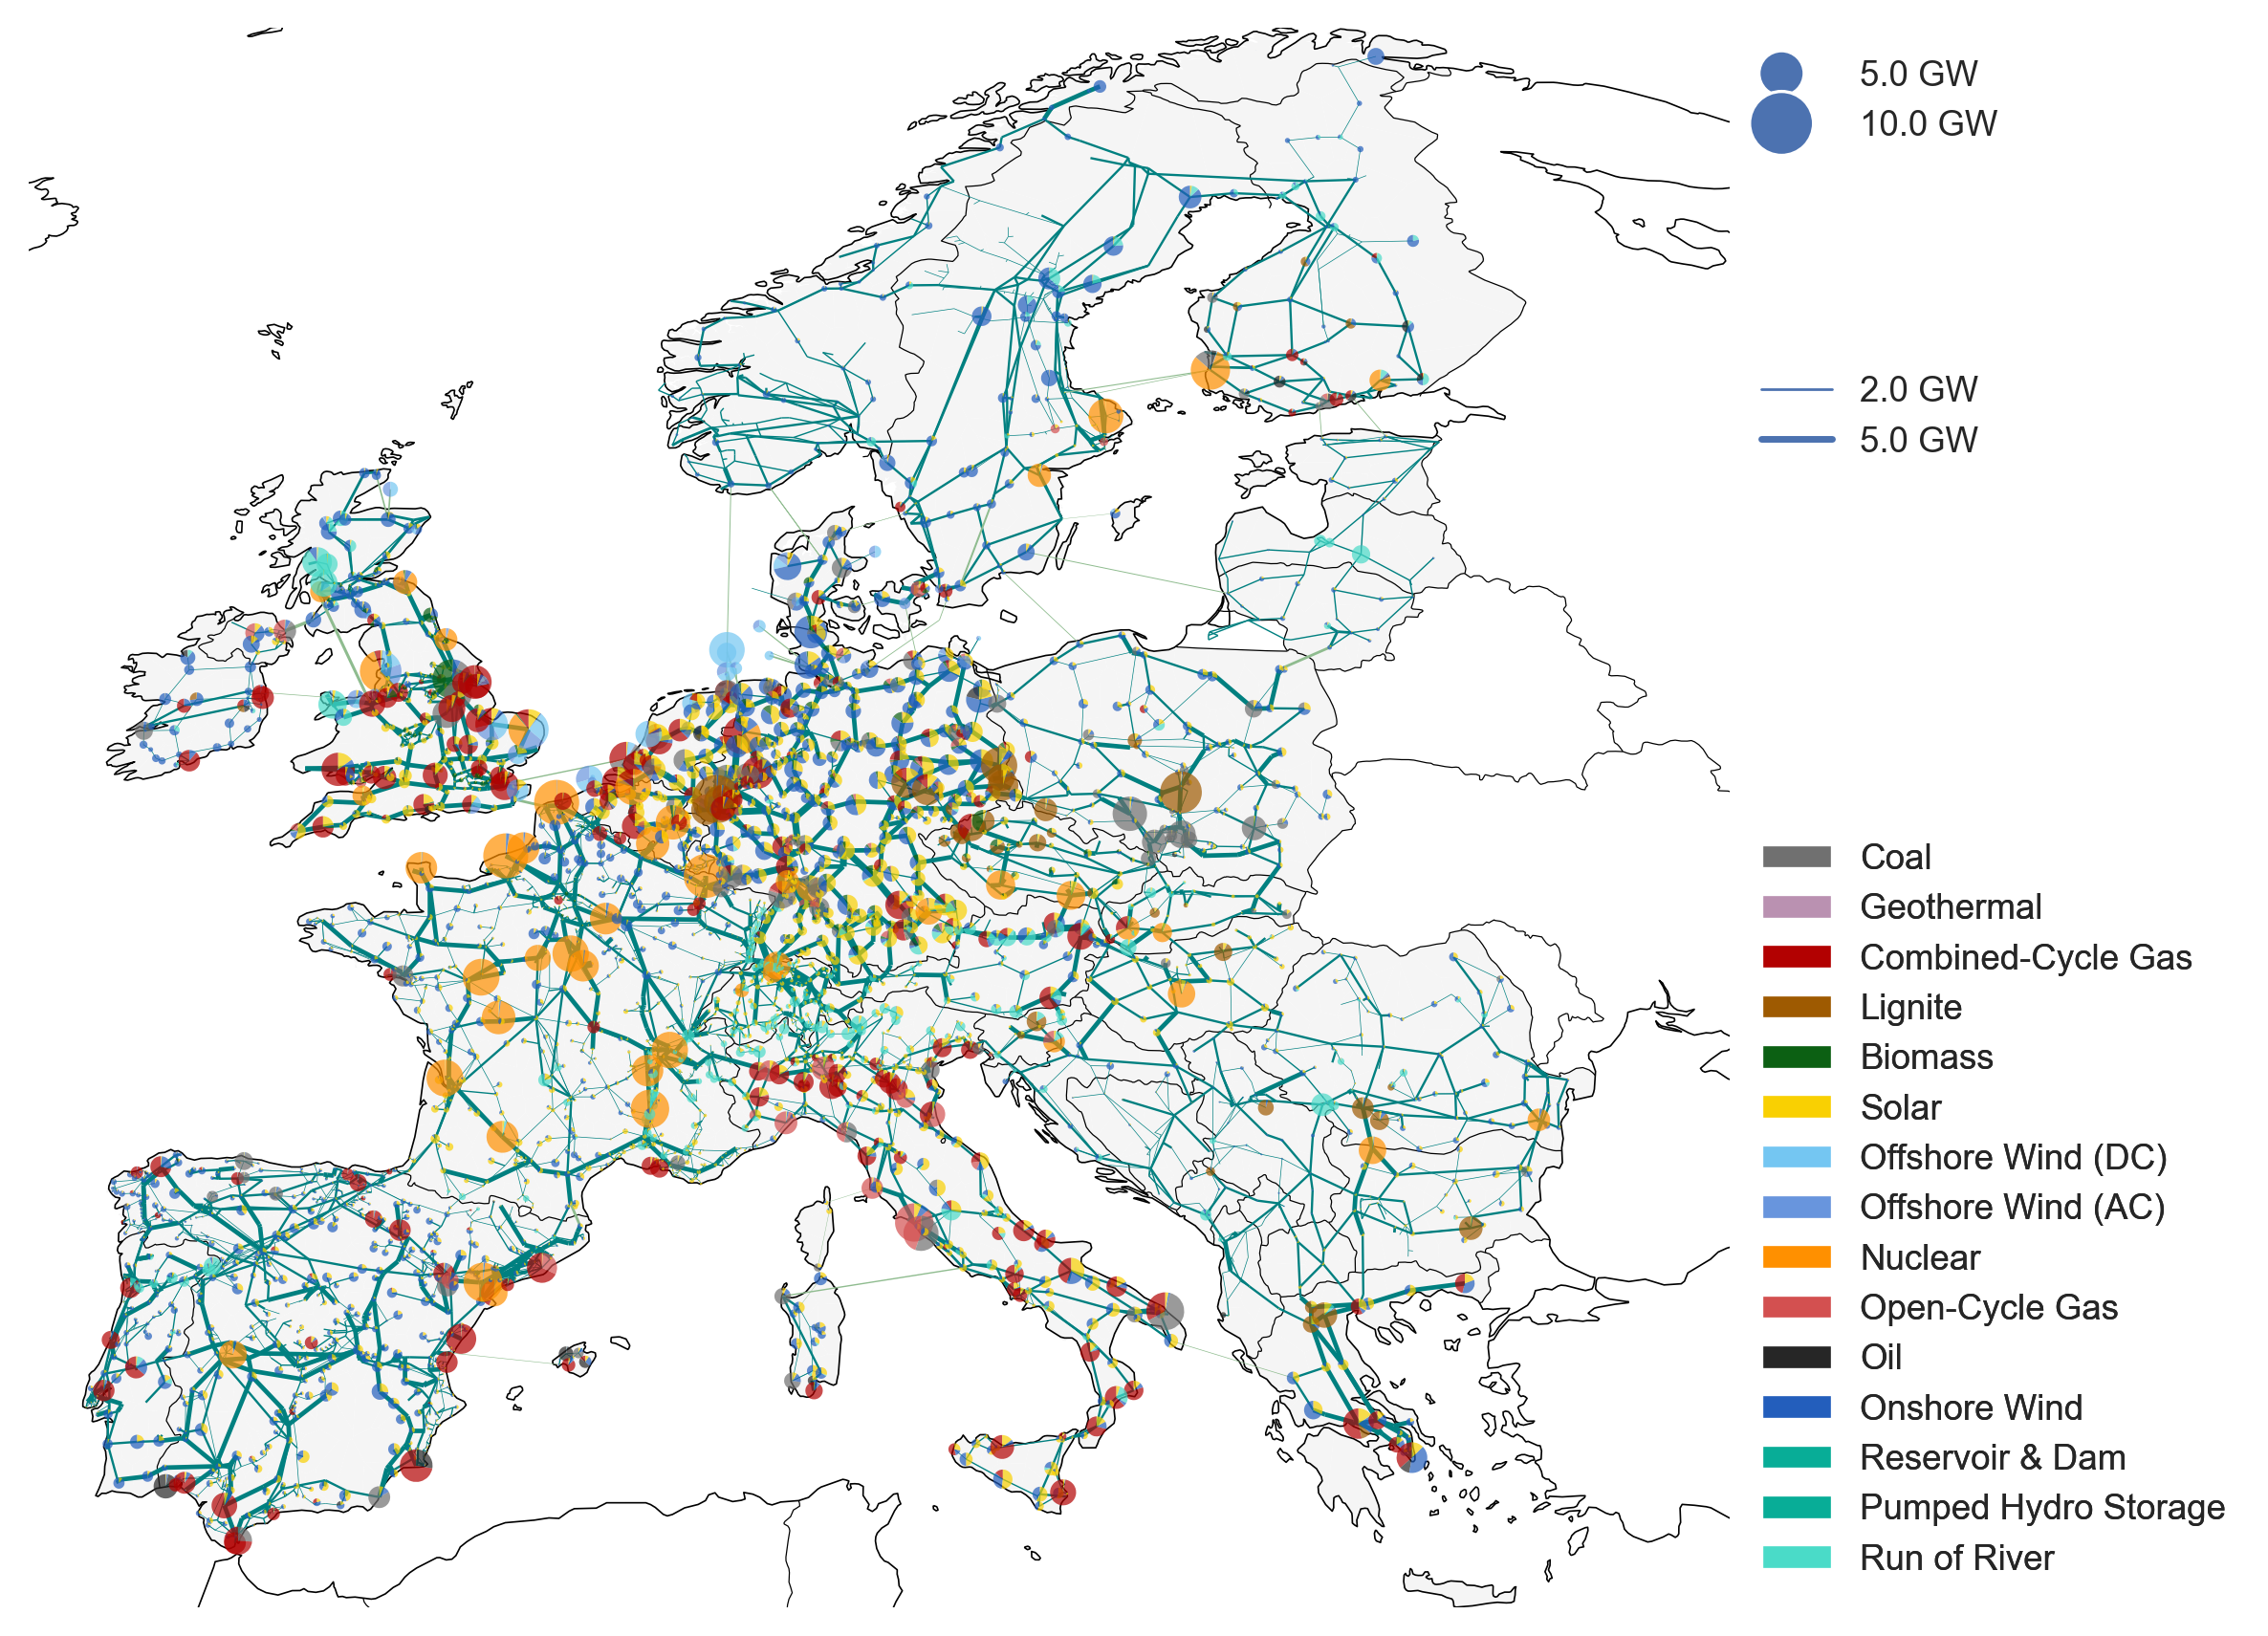
\includegraphics[width=1\linewidth]{elec.png}
  \captionof{figure}{Electricity high-voltage grid from AC 220 kV to 750 kV (UA) and DC 150 kV upwards. Option to include planned transmission projects.}
\end{center}\vspace{1cm}

\noindent
A \textbf{sector-coupled} extension adds demand and supply for the following sectors: transport, 
space and water heating, biomass, energy consumption in the agriculture, industry and 
industrial feedstocks, carbon management, carbon capture and usage/sequestration. This 
completes the energy system and includes all greenhouse gas emitters except waste 
management, agriculture, forestry and land use.

\begin{center}\vspace{1cm}
  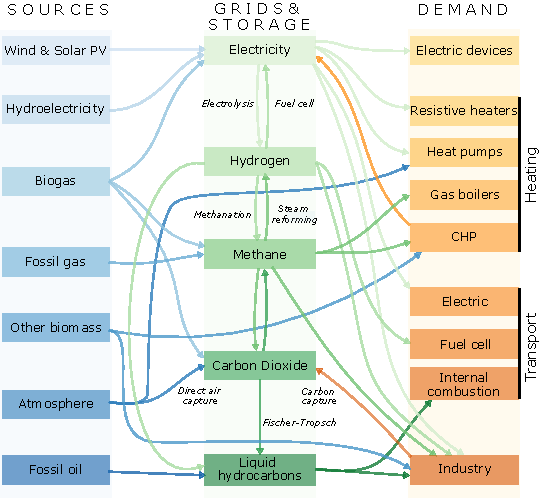
\includegraphics[width=0.7\linewidth]{multisector_figure.pdf}
  \captionof{figure}{Overview of the sectors in sector-coupled extension}
\end{center}\vspace{1cm}

\noindent
The generation of the model is controlled by the open workflow management system 
Snakemake \cite{Snakemake}. In a nutshell, the Snakefile defines a rule for each defined script, 
describing which files the scripts the scripts consume and produce 
(their corresponding input and output files). The snakemake tool then runs the scripts 
in the correct order according to the rules’ input and output dependencies. A \textbf{complete
data processing pipeline} is therefore generated, from the raw data to the results.

\vspace{2em}

\begin{tcolorbox}[width=0.95\linewidth,colback={conclusion},frame empty,boxsep=1cm]
\section*{Open Source}
  All tools are open-source and available on GitHub. The code is licensed under the MIT
  license, which allows for free use and modification of the code. 
  
  The framework packages are available on PyPI and conda-forge and can be installed using pip or conda.
\end{tcolorbox}    

\columnbreak

\noindent \textcolor{red100}{\huge \textbf{Toolbox}}
\\
\textit{Other Projects in the PyPSA Ecosystem}
\\

\noindent \textcolor{black}{\Large \textbf{linopy}}
\\
\textit{Linear ptimization with N-D labeled arrays in Python}
\vspace{0.5em}
\begin{center}
  
\includegraphics[width=15em]{linopy.pdf}
\end{center}
\vspace{0.5em}
linopy facilitates \textbf{optimization with real world data}. It builds a bridge 
between data analysis packages like xarray \& pandas and problem solvers like cbc, 
gurobi. linopy supports Linear, Integer, Mixed-Integer and Quadratic Programming while 
aiming to make linear programming in Python easy, highly-flexible and performant. \\

\noindent \textcolor{black}{\Large \textbf{atlite}}
\\
\textit{Calculate renewable power potentials and time series}
\vspace{0.5em}
\begin{center}
  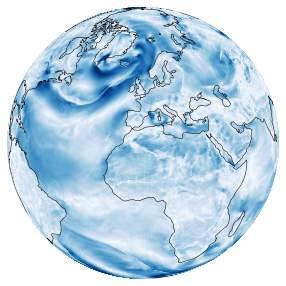
\includegraphics[width=12em]{atlite.png}
\end{center}
\vspace{0.5em}
atlite is a xarray-based Python library for \textbf{converting weather data into energy 
systems data}. It is designed to be lightweight, keeping computing resource 
requirements (CPU, RAM) usage low. It is therefore well suited to be used with big 
weather datasets. \\

\noindent \textcolor{black}{\Large \textbf{powerplantmatching}}
\\
\textit{Set of tools to combine multiple power plant databases}
\vspace{0.5em}
\begin{center}
  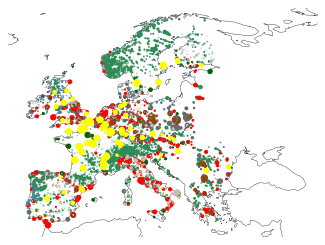
\includegraphics[width=12em]{powerplantmatching.png}
\end{center}
\vspace{0.5em}
powerplantmatching provides \textbf{ready-to-use power plant data for the European power system}. 
Starting from openly available power plant datasets, the package cleans, standardizes 
and merges the input data to create a new combined dataset, which includes all the 
important information. The package allows to easily update the combined data as soon 
as new input datasets are released.


%---------------------------------------------------------------------------------------
%	REFERENCES
%---------------------------------------------------------------------------------------
\singlespacing
\small
\nocite{*} % Print all references regardless of whether they were cited in the poster or not
\bibliographystyle{plain} % Plain referencing style
\bibliography{sample} % Use the example bibliography file sample.bib

%---------------------------------------------------------------------------------------

\end{multicols}
\end{document}